\section{Software}
Beschrieb was die Software machen soll und wie sie es machen soll!
Die Software soll die Stabilisierung der Temperaturen der Pumpdiode und des Kristall. 
Um die Versionierung der Softwarekomponenten aufrecht zu erhalten, wurde die Software \textit{Git} verwendet.

\subsection{Softwarespezifikation}
Analyse der Anforderungen, hier werden die verlangten Funktionen des Systems verstanden und Definiert. Für diese Software wurde eine inkrementeller Aufbau des Systems gewählt. So können im Nachhinein Anpassungen einfacher eingepflegt werden. $[6; S. 64-73]$

% \subsection{Softwareprototyp}
% \begin{enumerate}
%     \item Durchführbarkeitsstudie
%     \item Erhebung und Analyse der Anforderungen
%     \item Spezifikation der Anforderungen --> Als Liste realisieren(?)

%     \item Validierung der Anforderungen (Testen)
% \end{enumerate}
% 
% \begin{enumerate}
%     \item Entwickler- und Komponententests
%     \item Systemtests
%     \item Abnahmetests
% \end{enumerate}

% \subsection{Durchführbarkeitsstudie}
% Ein funktionierender Prototyp wurde bereits erstellt und die Daten konnten gelesen werden. Auch Befehle können an den Kontroller gesendet werden. Dies gewährleistet das senden der PID parameter, um den gewünschten Arbeitspunkt fest zu legen.

\subsection{Software Architektur}
% Hinweise auf die Objektorientierung der Software.
In diesem Kapitel wird die Architektur der Software beschrieben. Auf Grund der Wiederverwendbarkeit und der Übersicht des Programms wurde die Software möglichst modular aufgebaut. Sämtliche Teile der Software wurden in funktionelle Komponente unterteilt. Es wird zwischen dem Backend und dem Frontend unterschieden, wobei beide wiederum in kleinere Komponente unterteilt werden. Ebenfalls zur Übersicht wurde das Programm in einige Unterprogramme aufgeteilt. So wird sowohl die Ausführung des GUI und die Auswertung der Daten der TECs, als auch die Steuerung des Diodentreibers und die Ansteuerung des TEC-Treibers in jeweils eigenen Unterprogrammen ausgewertet.\\
Für die Sicherheit der bedienenden Person und der Komponenten des Laseraufbaus selber, mussten gewisse Sicherheitsvorkehrungen getroffen werden. Für das Einschalten der Diode, muss ein Schieber betätigt werden, ohne welchen die Freigabe zum Start des Diodentreibers nicht gewährleistet wird. Zusätzlich dürfen die TECs nicht mit zu viel Leistung betrieben werden, was zu deren Zerstörung führen könnte und dies auch die Diode in Mitleidenschaft ziehen könnte. Andererseits, muss verhindert werden, dass der der Diodentreiber zu viel Strom in den Laser einspeist. Die meisten dieser Vorkehrungen sind im Programmcodes untergebracht, andere mussten in der mitgelieferten Software der Komponenten eingestellt werden.

\subsection{Systemkontextmodell}
Das Systemkontextmodell beschreibt die anderen Systeme in der Umgebung und die Systemgrenzen. Der Aufbau des Kontrollers ist in Abbildung \ref{fig:systemkontextmodell} ersichtlich. $[6]$

\begin{figure}
    \centering
    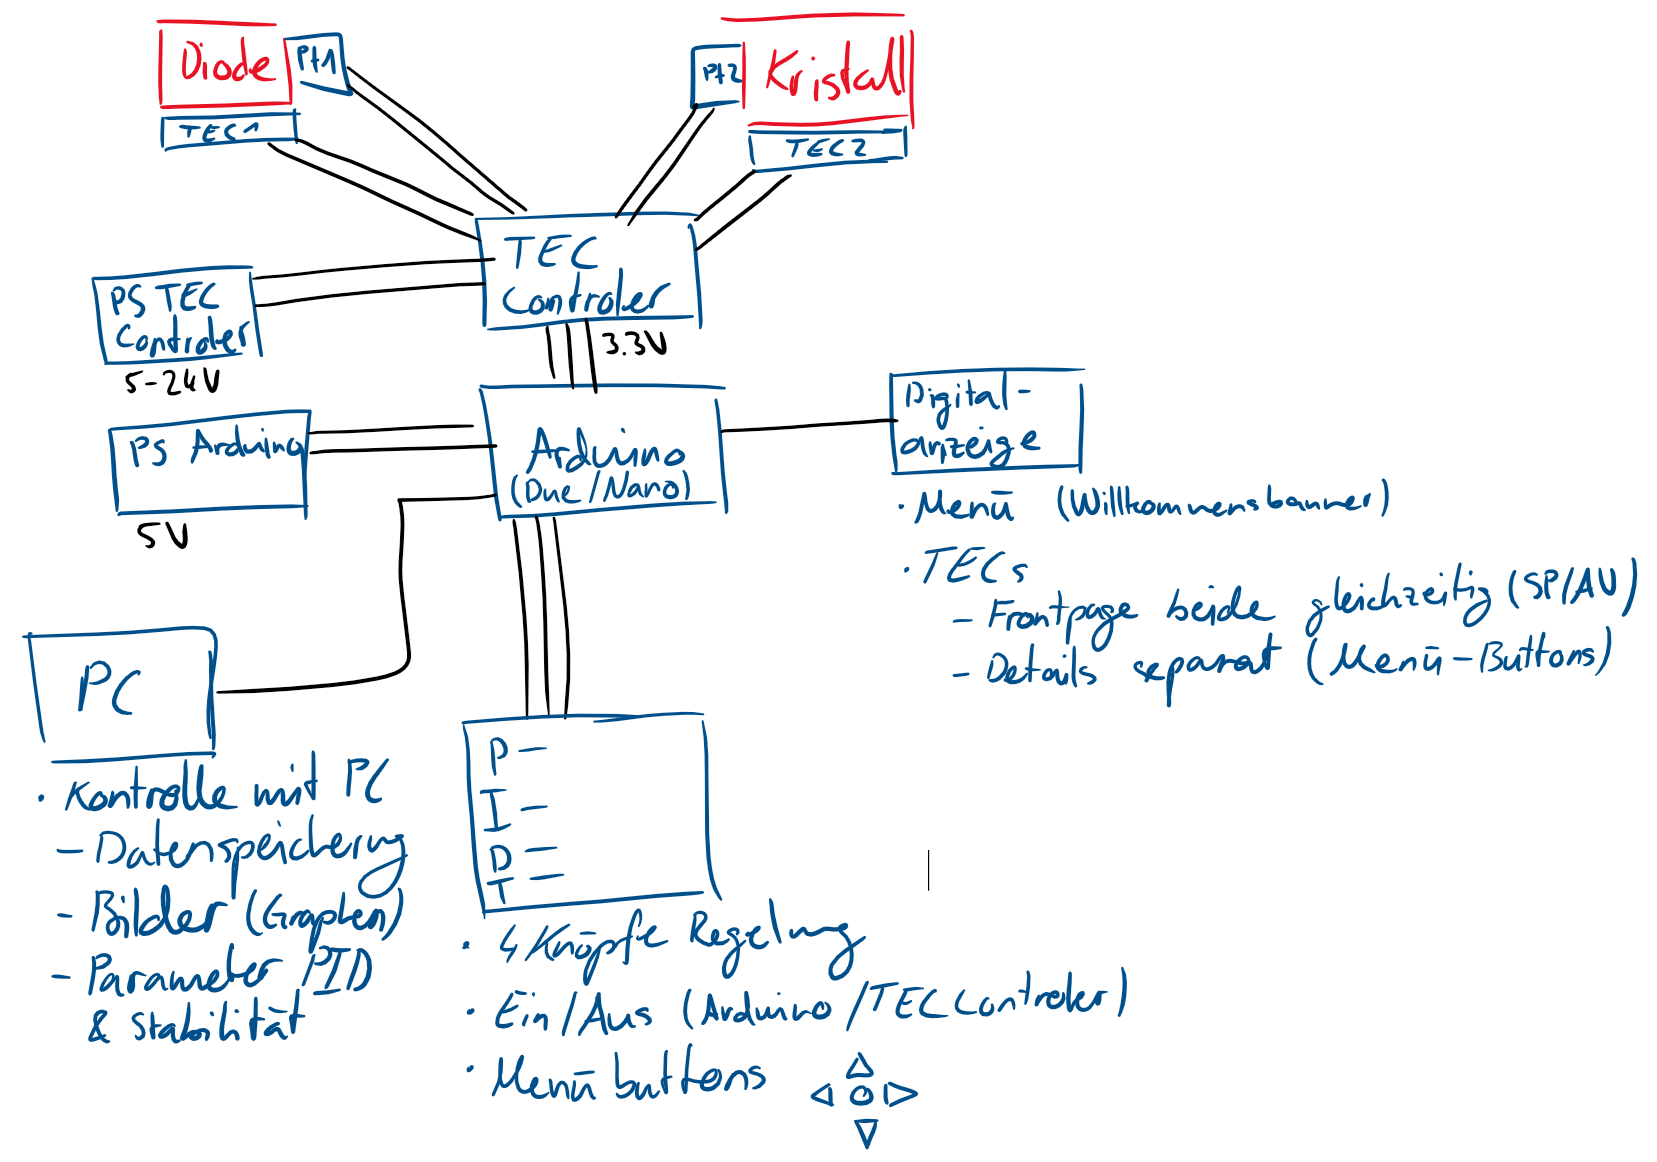
\includegraphics{98_images/scheme_wiring.PNG}
    \caption{Das Systemkontextmodell}
    \label{fig:systemkontextmodell}
\end{figure}

\subsection{Interaktionsmodell}
Das Interaktionsmodell zeigt auf, wie das System während der Benutzung mit seiner Umwelt zusammenspielt. Der Aufbau des Interaktionsmodells ist in Abbildung \ref{fig:interaktionsmodell}gezeigt. $[6]$

\begin{figure}
    \centering
    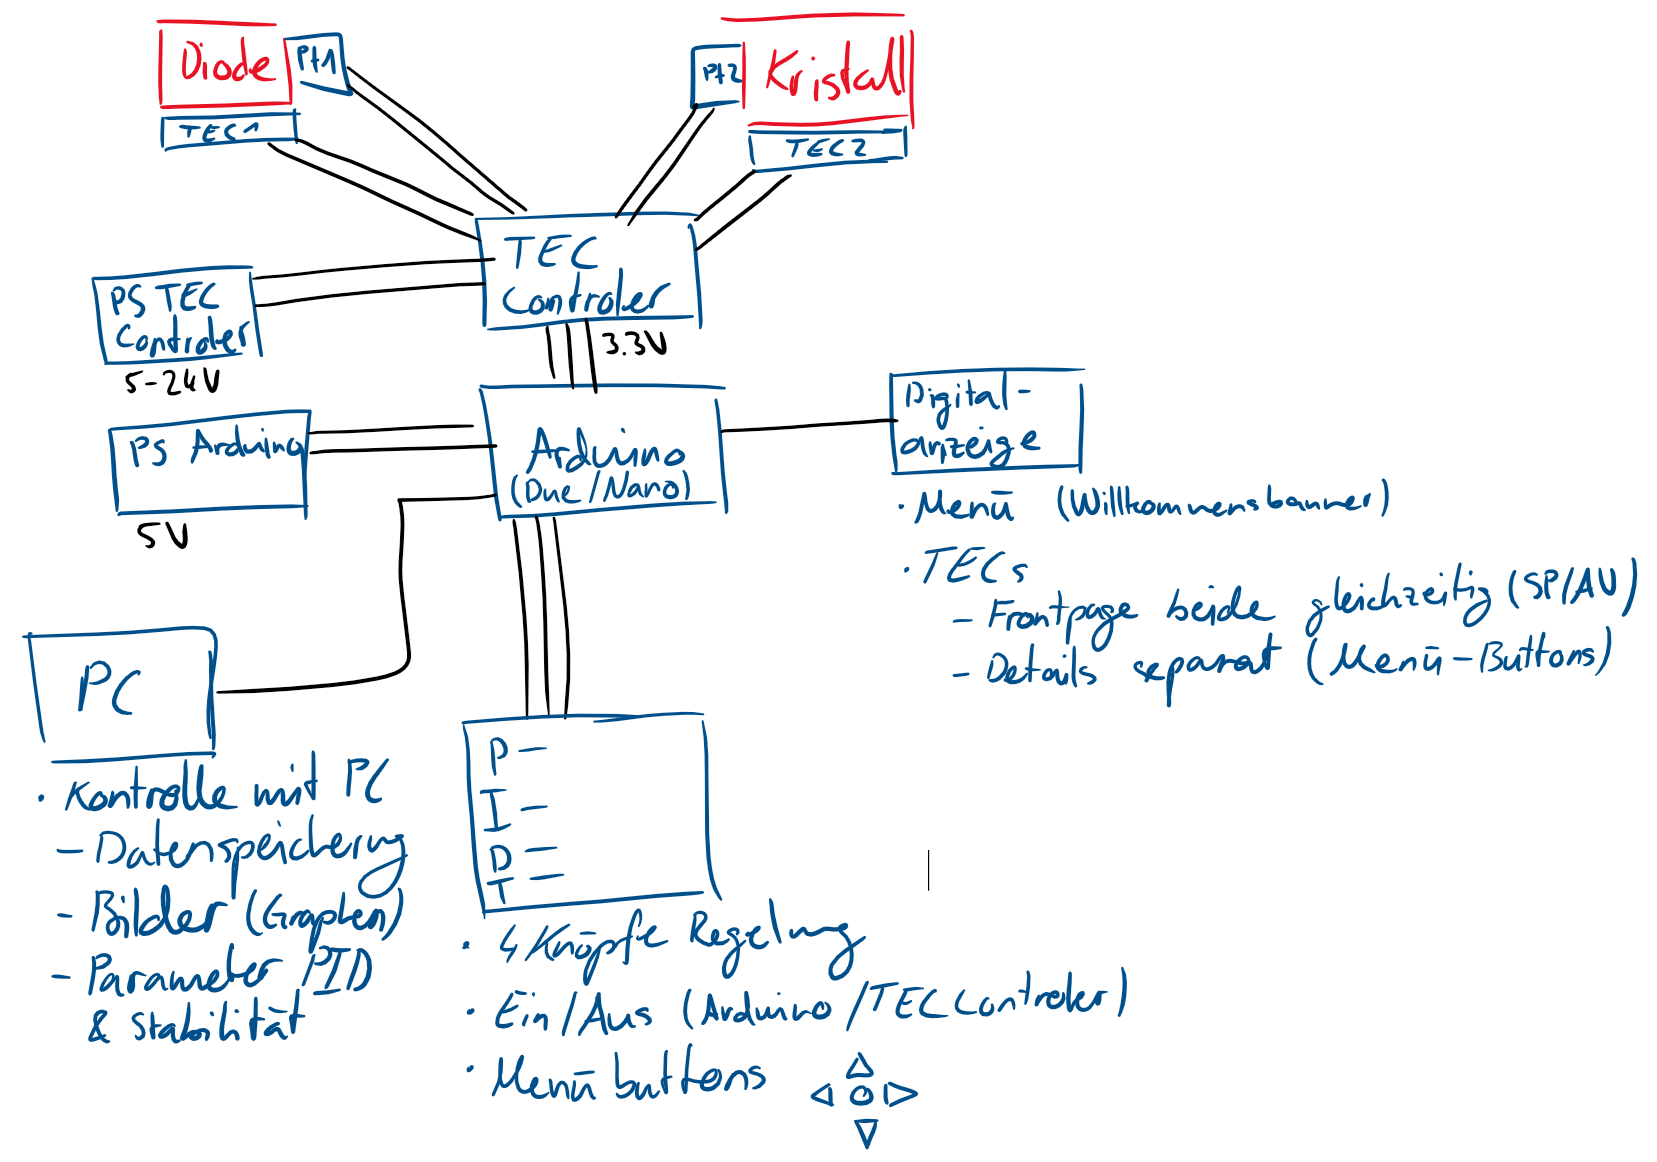
\includegraphics{98_images/scheme_wiring.PNG}
    \caption{Das Interaktionsmodell}
    \label{fig:interaktionsmodell}
\end{figure}

\subsection{Datenorientierte Modellierung}
Die Datenorientierte Modellierung wurde verwendet, um den gesamten Datenfluss im Kontroller fest zu halten. Der Datenfluss im Kontroller ist in Abbildung \ref{fig:dataflow_1} und in Abbildung \ref{fig:dataflow_2} gezeigt. $[6]$ S.170

\begin{figure}
    \centering
    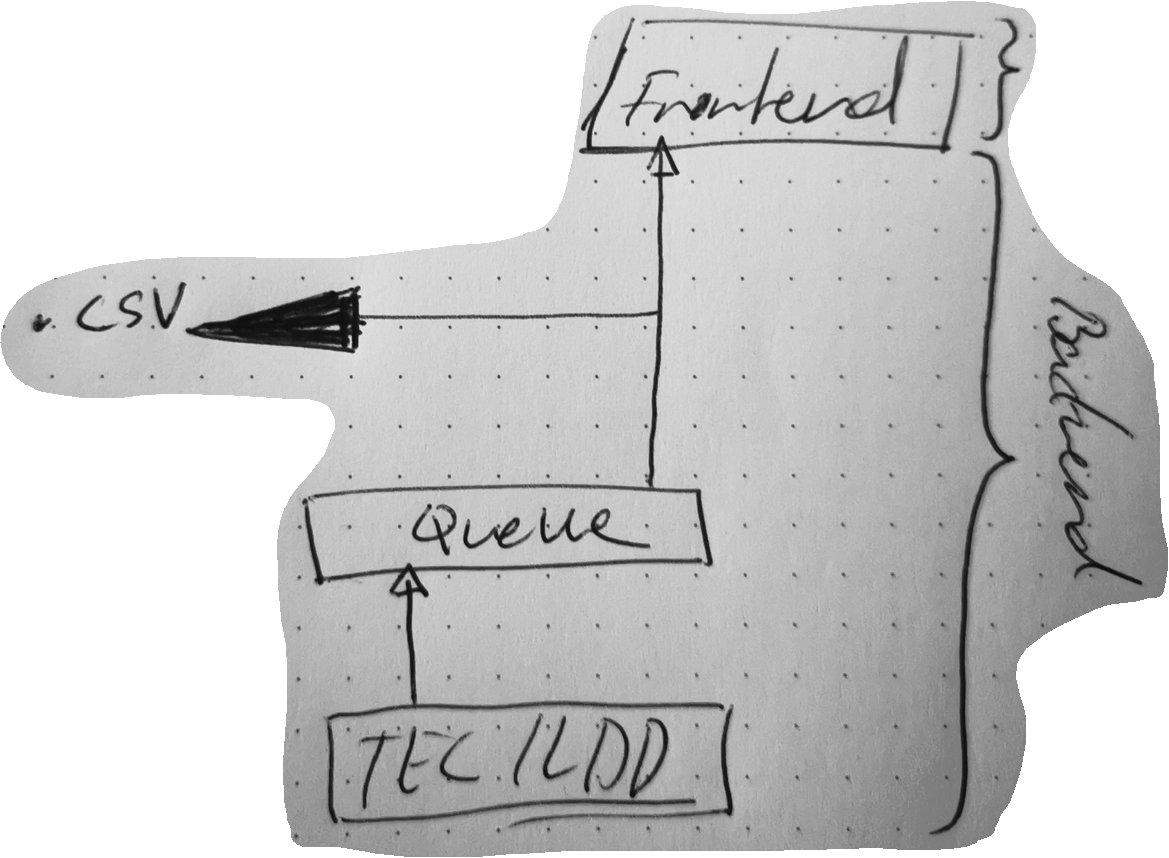
\includegraphics{98_images/data_flow_backend_frontend_tec_ldd.PNG}
    \caption{Hier ist der Datenfluss der Daten, die im Backend erzeugt werden ins Frontend dargestellt. Zu sehen ist die Queue, in die die Daten erst geschrieben werden und erst von den Konsumenten von da bezogen. Eine Abzweigung geht in die Datenbank im Hintergrund. Aus Gründen der Handlichkeit, wurde das Datenformat .csv verwendet. Dies ist mit weitverbreiteten Drittanbietersoftware wie Excel von Microsoft kompatibel und kann mit einer Grösse von über einer Million Zeilen eingelesen werden. Zusätzlich ist beim einfachen öffnen der Datei die Zeichensetzung für Menschen lesbar. }
    \label{fig:dataflow_1}
\end{figure}

\begin{figure}
    \centering
    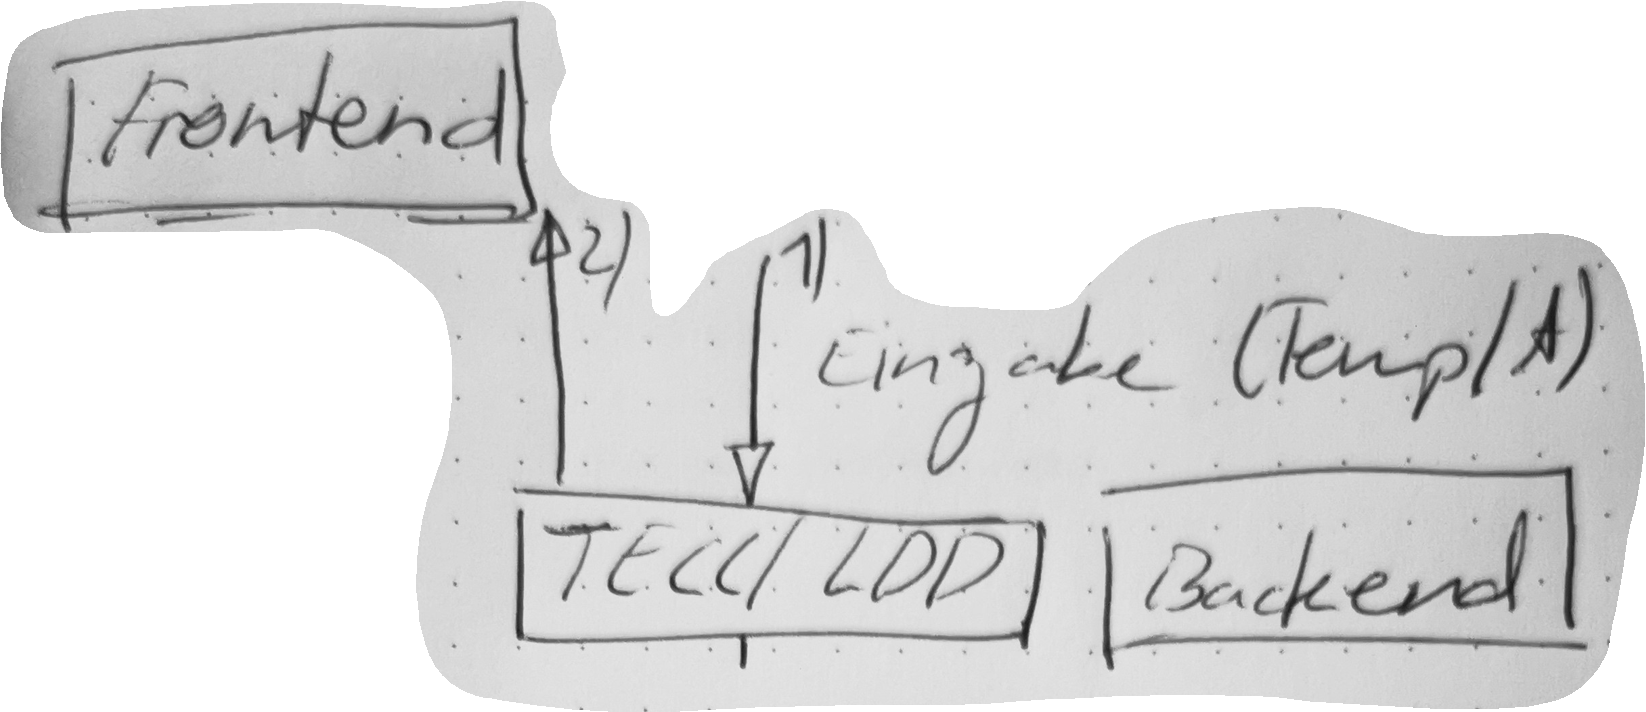
\includegraphics{98_images/data_flow_frontend_backend_tec_ldd.PNG}
    \caption{Hier ist der Datenfluss der Daten, die im Frontend erzeugt werden ins Backend dargestellt. Die Daten werden direkt und ohne in eine Queue geschrieben zu werden ins Backend und dann an die Kontroller (TEC-Treiber und Diodentreiber) weiter gereicht.}
    \label{fig:dataflow_2}
\end{figure}

\subsubsection{Das Producer-Consumer Design-Pattern}
\label{section:_producer_consumer}
Die Bereitstellung der Daten der TECs und des Diodentreibers sind nach dem \textit{Producer} \textit{Consumer}-Design-Pattern aufgebaut. Das System besteht aus einem Teilnehmer, der Daten zur Verfügung stellt und einem oder mehreren Teilnehmer, die diese Daten beziehen. Die Daten werden vom \textit{Producer}, dem Datenproduzent in eine Liste, die sogenannte \textit{Queue} geschrieben, und von da vom \textit{Consumer}, dem Datenbezüger ausgelesen. Das Schreiben und Lesen der Daten in der Queue folgt nach dem \textit{First-in First-out}-Prinzip, die Daten, die zuerst in die \textit{Queue} geschrieben werden, werden auch zuerst bezogen. Wird ein Datenpunkt aus der \textit{Queue} bezogen, wird dieser im selben Moment aus der \textit{Queue} gelöscht. Dies funktioniert stabil, auch wenn mit einem oder mehreren \textit{Threads} gearbeitet wird. $[7]$

\begin{figure}[H]
    \centering
    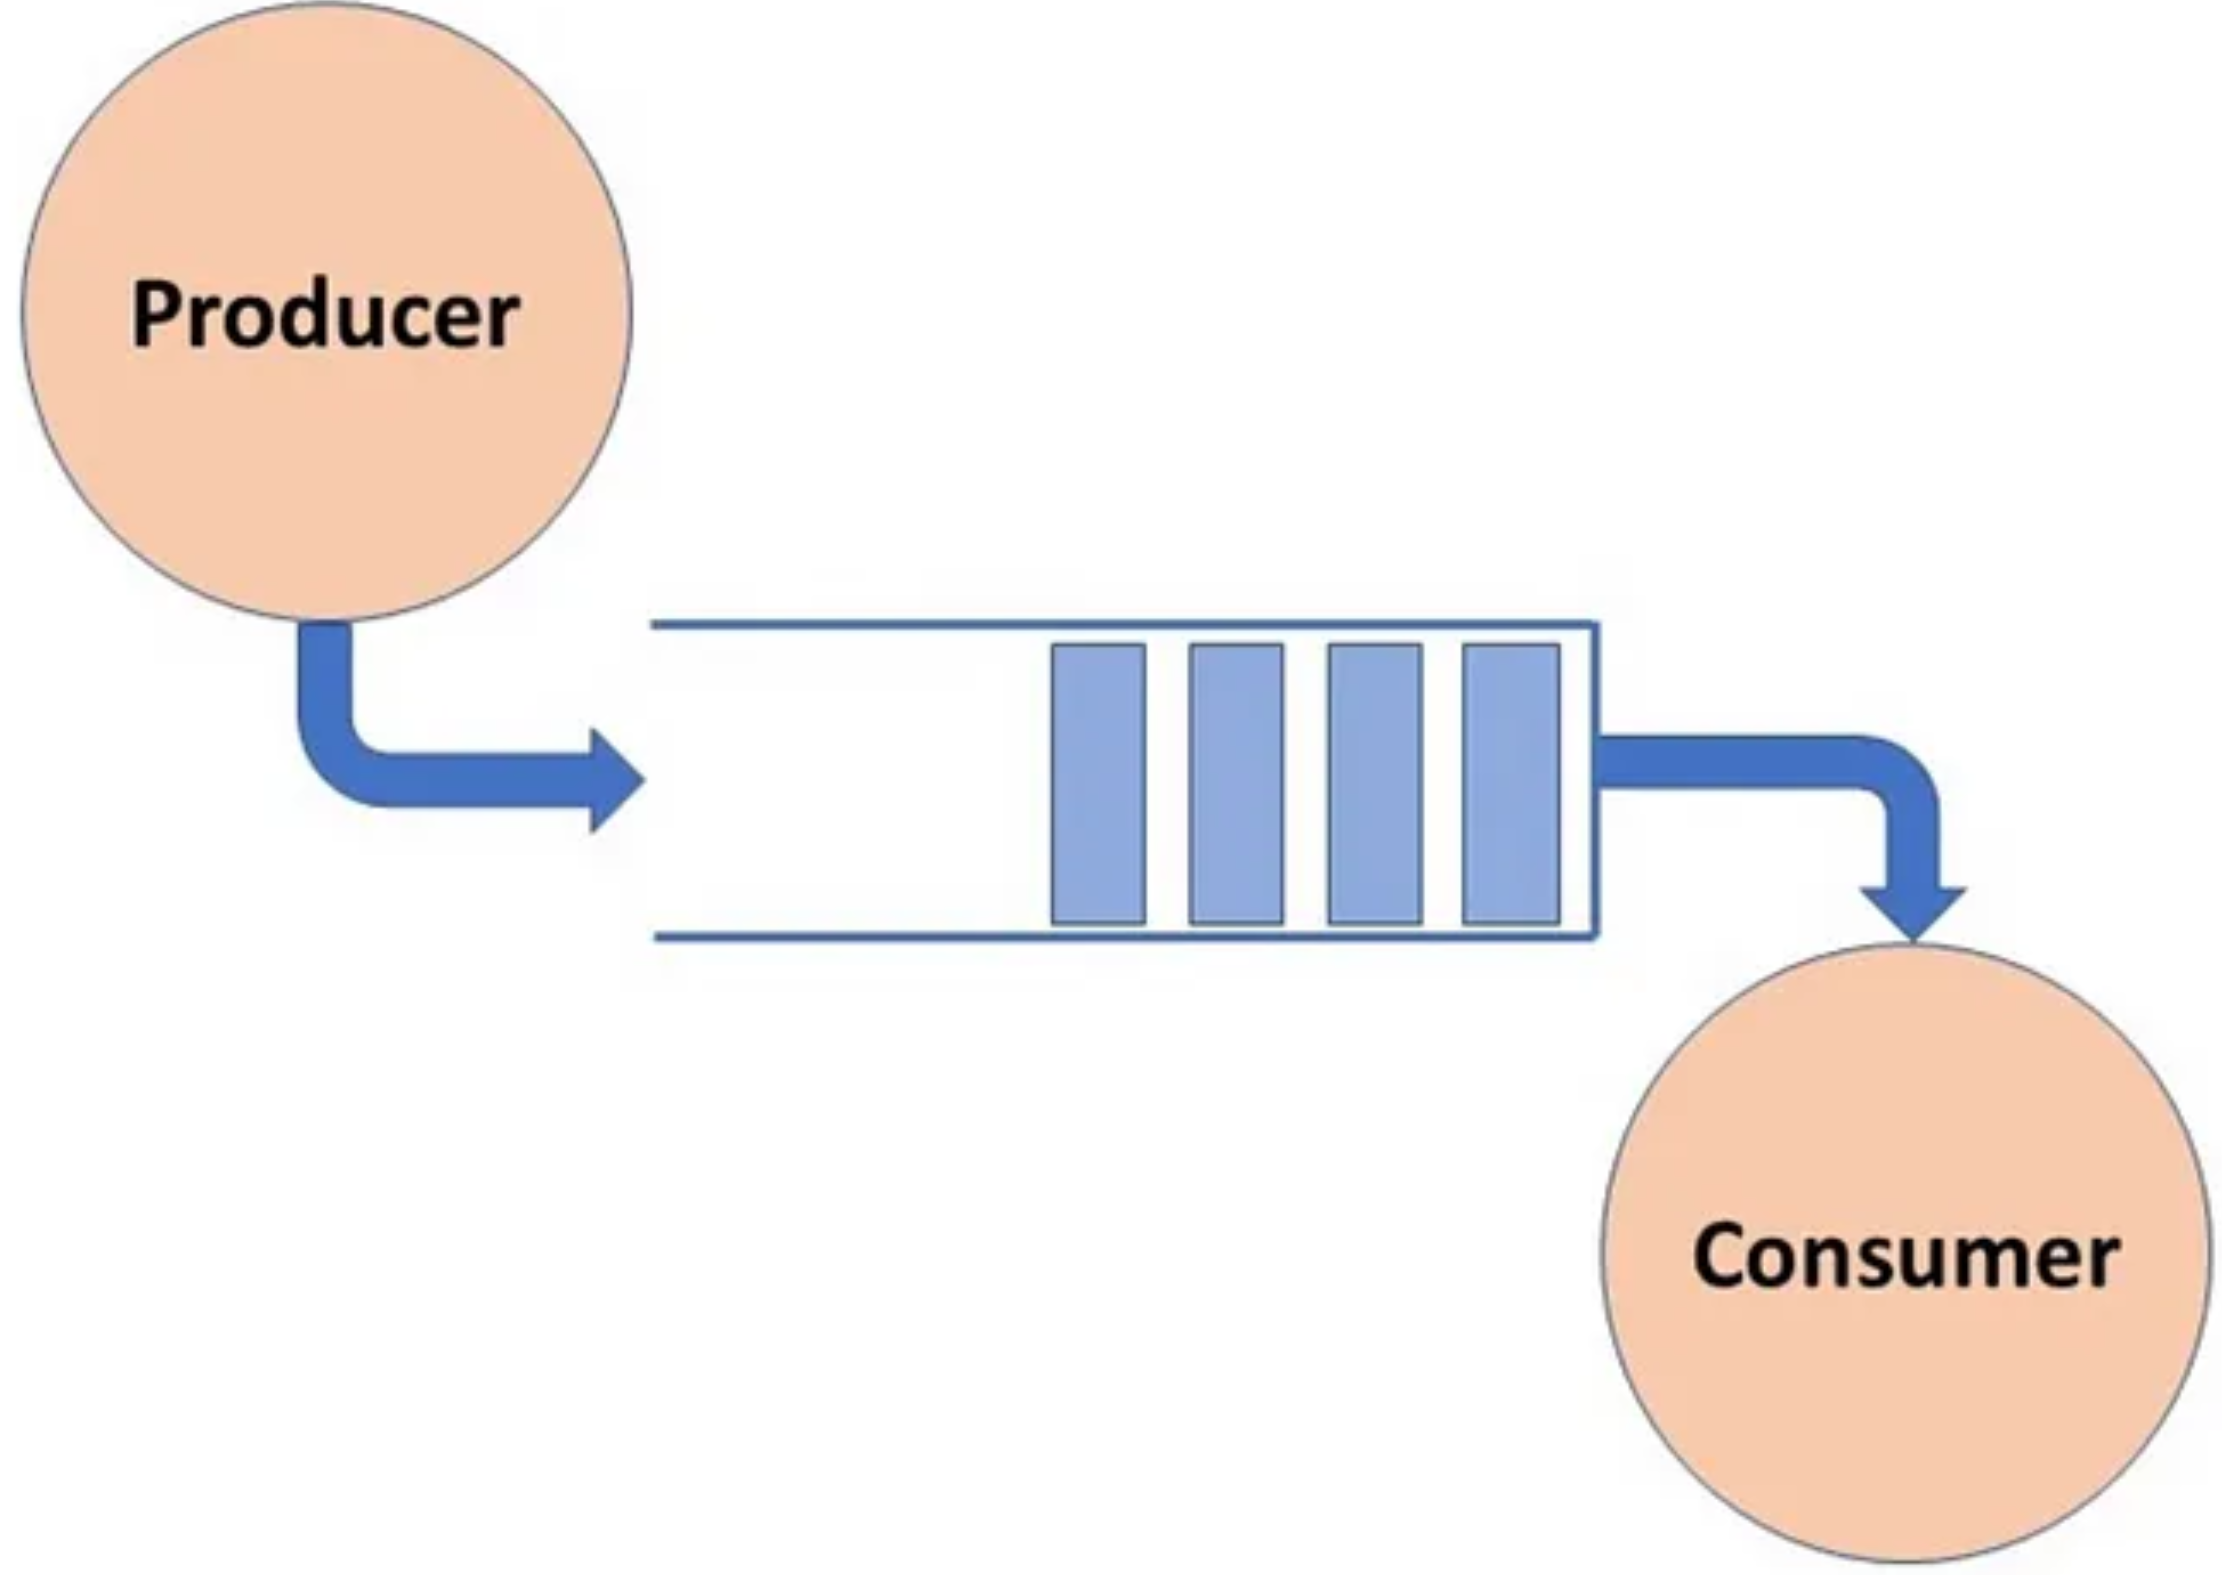
\includegraphics[scale=0.3]{98_images/producer_consumer_design_pattern.PNG}
    \caption{"Producer-Consumer" - Design Pattern; Der Datenproduzent fördert Informationen in die Queue, welche der Konsument bezieht.}
    \label{fig:_producer_consumer}
 \end{figure}

\subsubsection{Backend}
Das \textit{Backend} umfasst in der Softwareentwicklung alle Programmiertätigkeiten, die die Logik in einer Software ausmachen. So werden Kommunikation zu Kontrollern aufgebaut, Daten in Datenbanken gespeichert und Daten ans Frontend gesendet und auch von da bezogen.
Die von den Treibern produzierten Informationen werden in einer Datei im \textit{.csv}-Format abgespeichert und können so auf einem Drittsystem z.B. Microsoft Excel wieder verwendet und ausgewertet werden.

\subsubsection{Frontend}
Das \textit{Frontend} umfasst alle Bereiche, die mit der Benutzeroberfläche (GUI) zu tun haben. So beinhaltet dies das Framework, mit dem das Design der GUI entwickelt worden ist und deren Benutzerführung. 
Das graphische Benutzeroberfläche soll alle benötigten und wichtigen Werte anzeigen und einzustellende Werte einlesen. Darunter sind die Anzeige der Temperaturen des Kristalls und der Pumpdiode und, um die Zieltemperaturen zu halten. Daneben soll die Möglichkeit bestehen, den Nennstrom der Pumpdiode zu ändern. Neben den notwendigen angezeigten Werten, werden auch Werte zur Überwachung des Prozesses angezeigt. Um die Temperatur des Gehäuses zu überwachen, wird die Temperaturmessung des Prozessors des Raspberry PIs überwacht, mit der auf die Temperatur im Gehäuse der Steuerung geschlossen werden kann. Um den Anforderungen gerecht zu werden, wurden verschiedene Ansätze verfolgt die im Folgenden beschrieben werden. Dazu wurden Pro und Kontra vergleiche angestellt.

\textbf{Evaluierung des Frameworks}
Für die Realisierung der Benutzeroberfläche musste das Framework evaluiert werden, mit der die Benutzeroberfläche programmiert werden soll. Dafür werden die Frameworks \textit{Flask}, \textit{Tkinter} oder \textit{Customtkinter} eine Erweiterung von \textit{Tkinter} der Programmiersprache Python benutzt/verwendet. Dazu standen die Optionen Webbasiert (in einem Webbrowser verwaltbar und nutzbar) die andere Option ist eine Applikation. Beide Optionen laufen lokal auf dem Rechner (Raspberry PI 3B+), dabei steht die Leistung des Rechners im Vordergrund. Die vom TEC-Kontroller ausgelesenen Werte, werden im Sekundentakt an den Rechner gesendet und müssen innerhalb einer Sekunde ausgewertet werden können. Die Bedienung darf aus diesem Grund nicht zu viele Ressourcen des Rechners aufwenden. Dies konnte im Programm mit einer \textit{Queue} ein wenig abgefangen werden. Dazu ist es wünschenswert, wenn die Benutzeroberfläche zur einfacheren Handhabung die gesamte Anzeige ausfüllt. Folgend werden die Dafür bzw. Dagegen sprechenden Argumente aufgelistet.
Neben dem oben genannten Framework wurden auch Bibliotheken von Drittanbietern, die nicht nativ in der Installation von Python vorhanden sind verwendet. Die Beschreibung derer sind in Kapitel \ref{section:_libraries_py}.


\begin{table}[H]
    \centering
    \begin{tabular}{l|l|l|l}
        $-$&                        \textbf{Webbasiert}&        \multicolumn{2}{c}{\textbf{Applikation}}\\
        \hline
        \textbf{Kriterium}&         \textbf{Flask}&             \textbf{Tkinter}&           \textbf{Customtkinter}\\
        \hline
        Leistungseinbusse&          $=$ Mittel&                 $=$ Mittel&                 $=$ Mittel\\
        Schwierigkeitsgrad&         $-$ Mittel - Schwierig&     $+$ Einfach - Mittel &      $+$ Einfach - Mittel \\
        Bibliothek&                 $-$Standard&                $+$ Standard &              $+$ Standard \\
        Design&                     $+$ Vielfältig, schöner&    $-$ Weniger vielfältig &    $+$ Vielfältig\\
        Erfahrung&                  $-$ Keine Erfahrung&        $+$ Bereits Erfahrung &     $+$ Ähnlich Tkinter\\
        Programmiersprachen&        $-$ Python und HTML&        $+$ Python &                $+$ Python \\
    \end{tabular}
    \caption{Evaluierung des Frameworks zur GUI Programmierung. Gelistet sind die Namen der jeweiligen Frameworks. \textit{Flask} ist das Framework der webbasierten Umgebung, wohingegen \textit{Tkinter} und \textit{Customtkinter} eigene Applikationen sind.}
    \label{tab:gui_programming}
\end{table}

Aus den Gründen der Erfahrung und der Anwendbarkeit mit Tkinter, fiel die Entscheidung auf die App-Variante. Zusätzlich konnte mit dem \textit{Customtkinter} Framework modernere Designs kreiert werden. Dies soll die Nutzung der Oberfläche vereinfachen. Es können ergonomische und ansprechende Designs realisiert werden.

\textbf{Benutzerführung}
Beschreibung, wie im Menü navigiert wird, Architektur des Menüs. Hier sollen auch die verschiedenen Modi dokumentiert werden. Namentlich "Initialisierung", "Ready", "Eingabe Parameter". Sind die Netzwerk Voraussetzungen gegeben,  kann zusätzlich der Rechner über einen Fernzugriff gesteuert werden. [Annex 2]

\subsubsection{Kommunikation zwischen Backend - Frontend}

\begin{itemize}
    \item Mit welchen mitteln werden die Informationen aus dem Backend im Frontend angezeigt
    \item Kommunikation Raspberry PI - Digitalanzeige
    \item Kommunikation Raspberry PI - TECs
\end{itemize}

% \subsection{Funktionalitätstest}
% Erstellen einer Tabelle im Vorhinein, um die Funktionalitäten der Software zu testen.
% Wie in einem Change Request auf der Testseite.

\subsection{Testen der Software}
Zur Überprüfung der Funktionalität der Software und der Hardware wurde zuerst ein Test definiert. Dieser Test unterliegt der Anforderungsspezifikation und soll die Erfüllung der Funktion der Software und Hardware gewährleisten.

\begin{itemize}
    \item Probleme beschreiben und Abgrenzen; Was sind die Ziele für die Software
    \item Menü für die Handhabung und Einstellungen
\end{itemize}

Für den zwei-kanaligen TEC-Kontroller wurde ein Treiber des Unternehmens Meerstetter Engineering AG gewählt. Dieser erfüllte alle Spezifikationen, die für die Funktionalität des Systems benötigt wurden. Daneben kann es die PID-Parameter automatisch wählen und müssen nicht noch im Steuerungsprozess evaluiert werden. Die Zweikanaligkeit des Kontrollers kann simultan das Peltierelement des Kristalls als auch dies der Pumpdiode steuern.


\textbf{Romain Caretto's Vorarbeit erwähnen}
\textbf{Neuster Stand der Technik}
\textbf{Mit welcher Methode zum Ziel; der letzte Paragraph der Einleitung Inhaltsverzeichnis im Prosa}
% Und noch schnell die ganze Bibliographie zitieren:
\nocite{*}

% \subsection{Theorie 1}
% 
% \emph{Informieren und orientieren.} Das Schema in Abbildung~\ref{fig:software_struktur} enthält \ldots, \lipsum[7-7]
% 
% \begin{figure}[b]
% \begin{center}
% 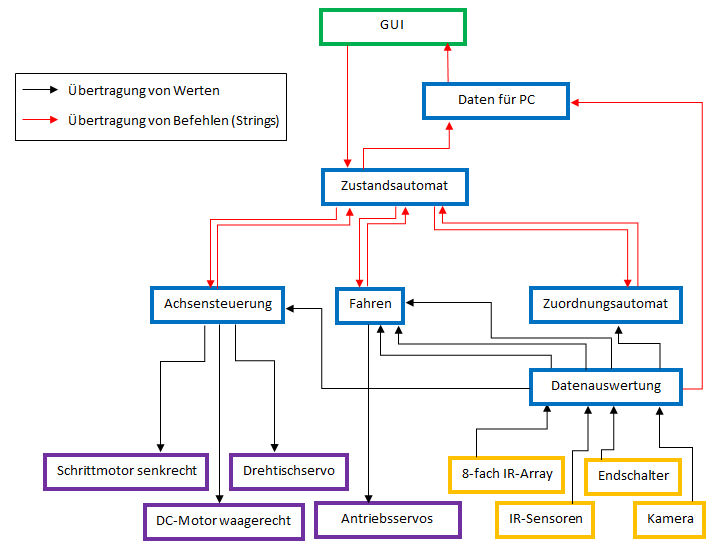
\includegraphics[width=\linewidth]{software_struktur.png}
% \end{center}
% \caption{Realisierte Software-Struktur in LABView}
% \label{fig:software_struktur}
% \end{figure}
% 
% \subsection{Unterkapitel}
% 
% \lipsum[8]  Nach Formel \eqref{eq:sincos}:
% \begin{equation}
% \sin \alpha \pm \sin \beta = 2\sin\frac{\alpha\pm\beta}{2}\cos\frac{\alpha\mp\beta}{2}\,. \label{eq:sincos}
% \end{equation}
% 
% \lipsum[9]
% \begin{equation}
% x = \frac{-b\pm\sqrt{b^2-4ac}}{2a}\;.
% \end{equation}